\section{Cálculos}


\begin{enumerate}
        \item Expresar la ley de velocidad para la reacción.
         Para este caso $ A$ es acetato de etilo y $B$ es el Hidróxido de sodio.

                $$ -r_{a}= k[A][B] $$
        \item Elaborar una gráfica de conductividad en función del tiempo y 
        extrapolar a t = 0.

     \begin{figure}[H]
         \centering
         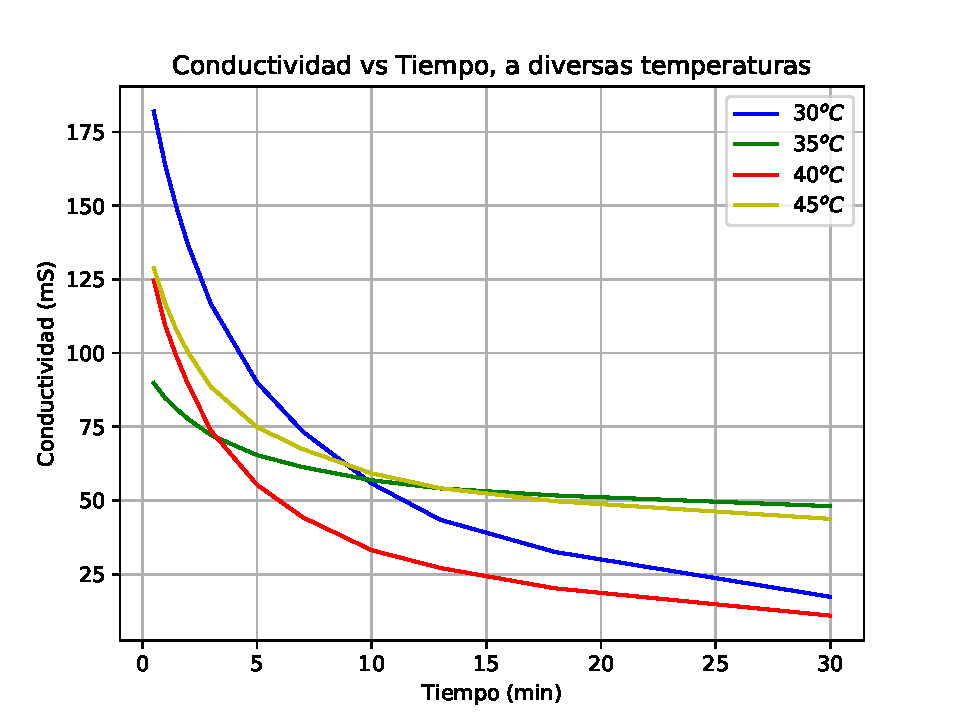
\includegraphics[scale = 0.8]{Figuras/Conductividad_vs_Tiempo.pdf}
         \caption{Diagrama de la pr\'{a}ctica}
      \end{figure}

      \item Plantear las ecuaciones de conductividad en función del tiempo.
       A partir de estas ecuaciones, determinar las concentraciones de los productos 
       que se han formado a cualquier tiempo t, en función de la conductividad.\\
      Con los siguientes  datos se elabora una gráfica de calibración para obtener 
      las concentraciones a cualquier tiempo.

% Table generated by Excel2LaTeX from sheet 'Hoja1'
\begin{table}[H]
  \centering
  \caption{Datos de la práctica}
    \begin{tabular}{crrrr}
    \hline
    \multicolumn{1}{l}{Temperatura} & $30 \: C^{ \circ}$    & $35\: C^{ \circ}$    & $40\: C^{ \circ}$    & $45\: C^{ \circ}$ \\
    \multicolumn{1}{c}{\multirow{2}[0]{*}{Tiempo}} & \multicolumn{1}{p{4.335em}}{Conducti} & \multicolumn{1}{p{4.445em}}{Conducti} & \multicolumn{1}{p{4.28em}}{Conducti} & \multicolumn{1}{p{3.945em}}{Conducti} \\
          & \multicolumn{1}{p{4.335em}}{vidad(mS)} & \multicolumn{1}{p{4.445em}}{vidad(mS)} & \multicolumn{1}{p{4.28em}}{vidad(mS)} & \multicolumn{1}{p{3.945em}}{vidad(mS)} \\ \hline
    0.5   & 181.95 & 89.82 & 124.65 & 128.8 \\
    1     & 163.65 & 84.74 & 109.24 & 116.77 \\
    1.5   & 149.17 & 80.97 & 98.64 & 107.59 \\
    2     & 136.56 & 77.64 & 89.3  & 100.18 \\
    3     & 116.54 & 72.14 & 73.6  & 88.49 \\
    5     & 90.12 & 65.4  & 55.33 & 74.91 \\
    7     & 73.36 & 61.31 & 44.29 & 67.42 \\
    10    & 55.79 & 56.87 & 33.14 & 59.22 \\
    13    & 43.44 & 54.1  & 27.1  & 54.17 \\
    18    & 32.54 & 51.72 & 20.2  & 49.76 \\
    30    & 17.33 & 48.08 & 10.95 & 43.78 \\ \hline
    \end{tabular}%
  \label{tab:addlabel}%
\end{table}%
  

        \begin{figure}[H]
            \centering
            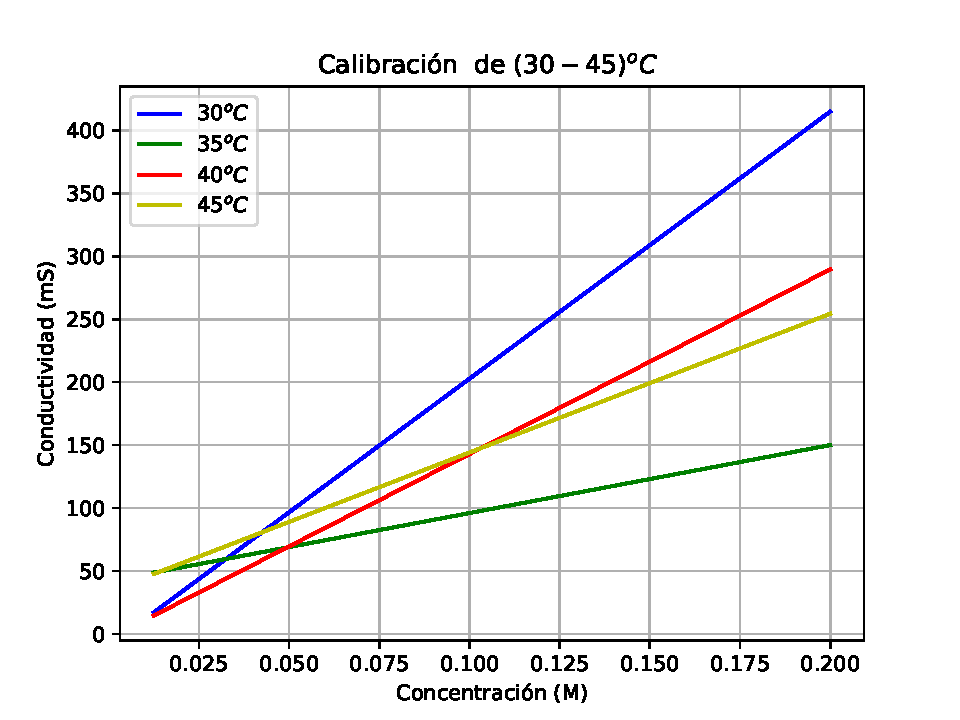
\includegraphics[scale = 0.8]{Figuras/calibracion_todos.pdf}
            \caption{Diagrama de la pr\'{a}ctica}
        \end{figure}

    Con esta gráfica se tiene el ajuste de polinomio:
            $$  Conductividad = m[x] + b$$

\begin{figure}[H]
    \centering
\begin{tabular}{cccc}
\hline
$ T (^{\circ}$C) & Pendiente (m) & Intercepto & $r^{2}$ \\
\hline
30 & 2122.7 & -9.5334  & 1   \\
35 & 540.32 & +41.936  & 1   \\
40 & 1467.2 & -3.84    & 1   \\
45 & 1102.7 & +33.813  & 1   \\
\hline

\end{tabular} 
\caption{Datos  de calibración }
    \label{fig:my_label}
\end{figure}


\end{enumerate}


\begin{figure}[H]
    \centering
    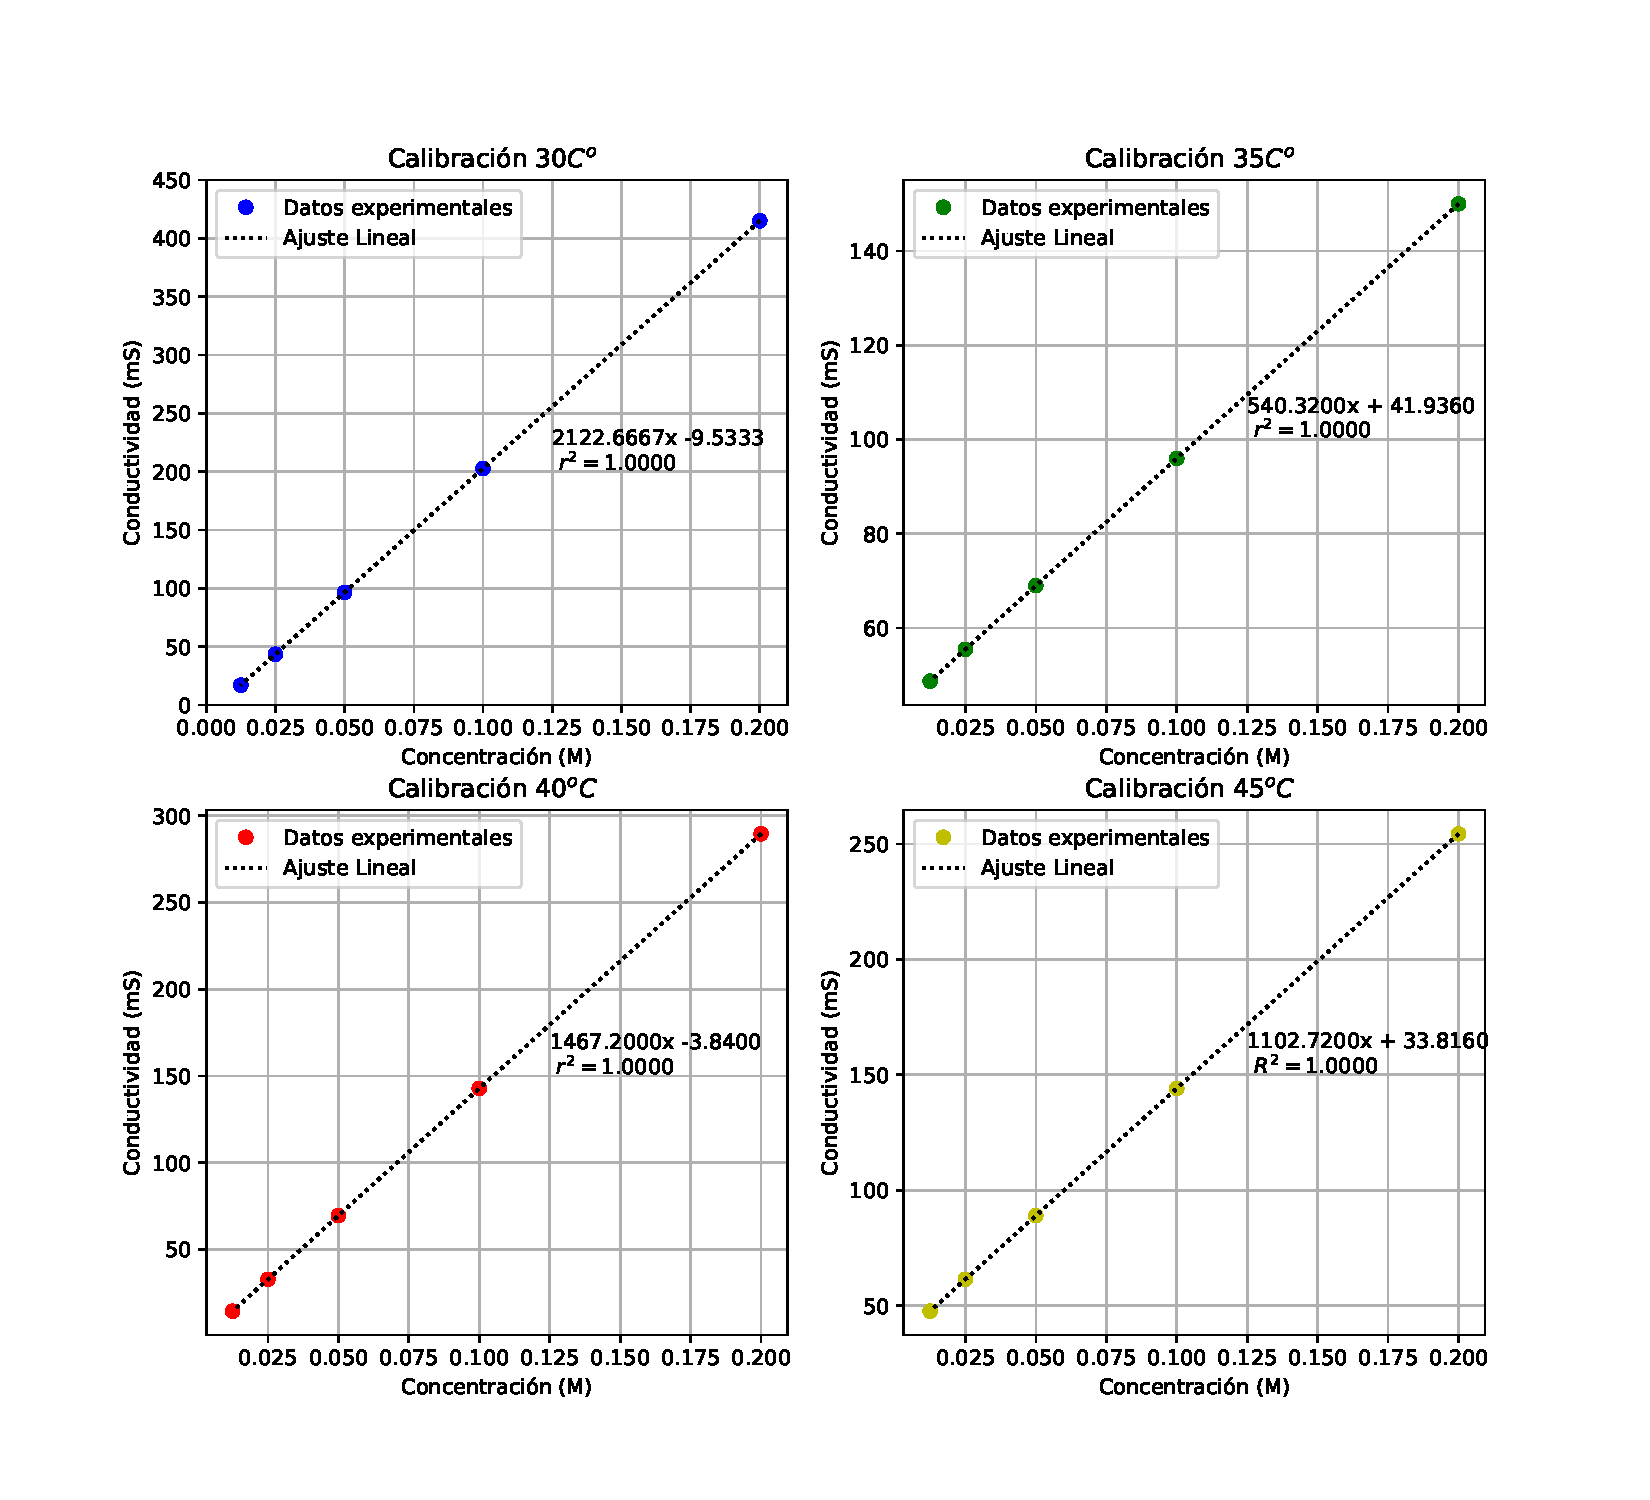
\includegraphics[scale=0.65]{Figuras/FiguraTodos.pdf}
    \caption{Diagrama de la pr\'{a}ctica}
\end{figure}

\begin{figure}[H]
    \centering
    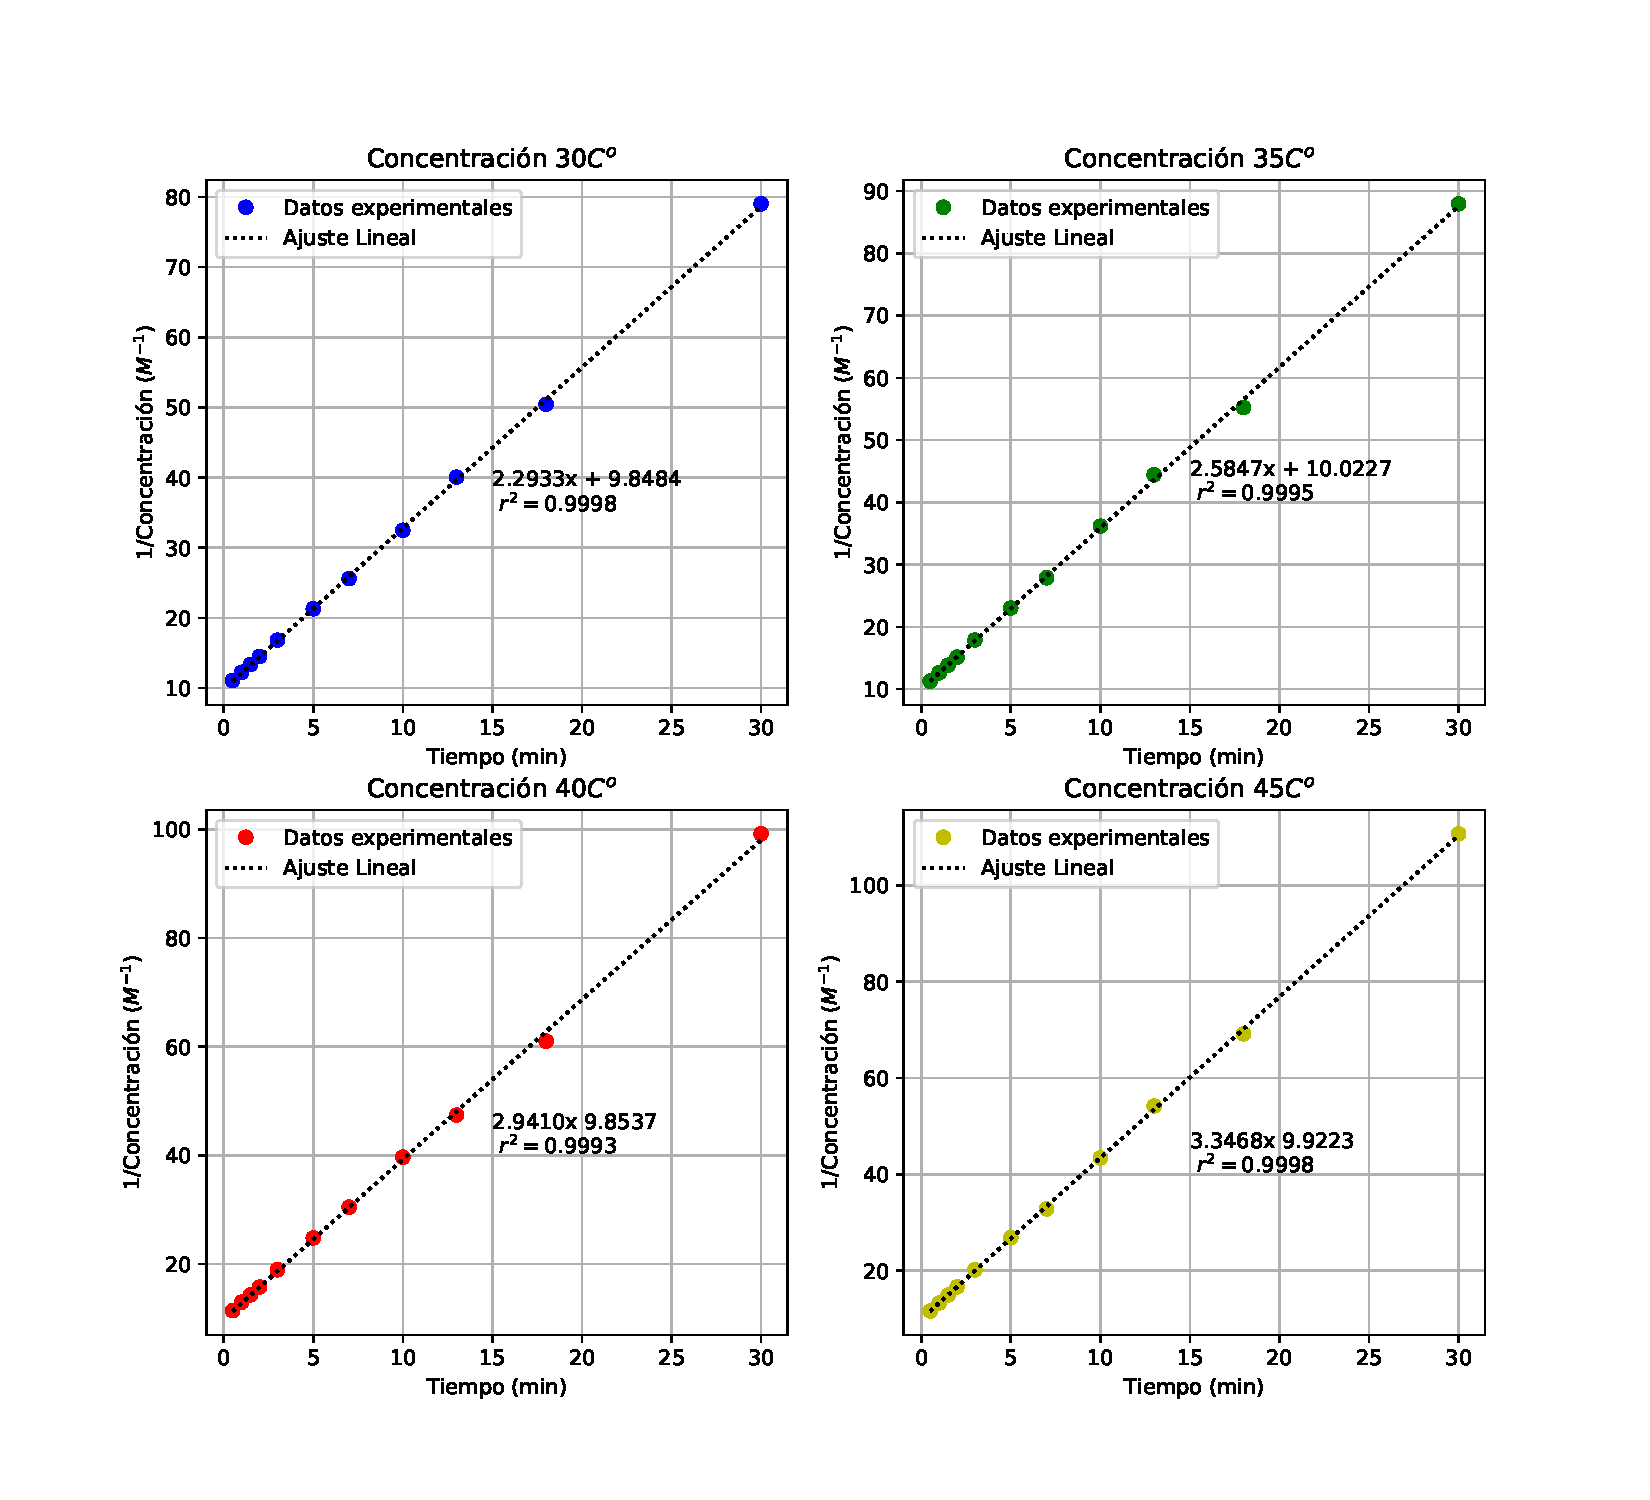
\includegraphics[scale=0.65]{Figuras/Ctodos.pdf}
    \caption{Diagrama de la pr\'{a}ctica}
\end{figure}

\begin{figure}[H]
    \centering
    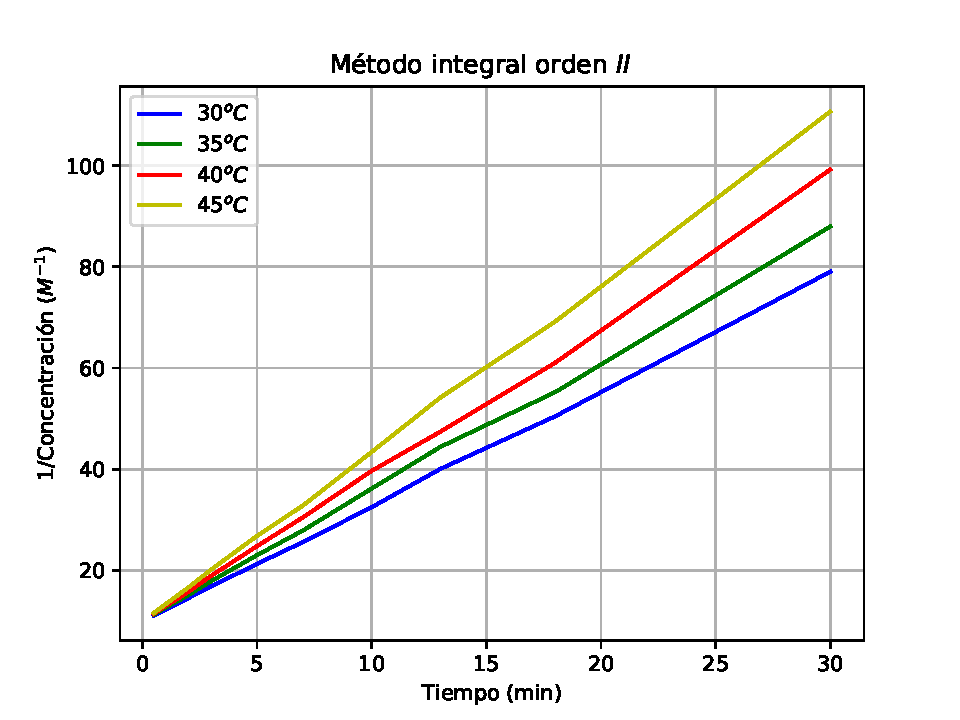
\includegraphics[scale=1]{Figuras/concentracion_todos.pdf}
    \caption{Diagrama de la pr\'{a}ctica}
\end{figure}


